\documentclass[11pt,a4paper]{article}
\usepackage[margin=2.3cm]{geometry}
\usepackage{amsmath,amssymb,amsthm}
\usepackage{graphicx,booktabs,caption,subcaption}
\usepackage{microtype,enumitem,float,multirow}
\usepackage[table]{xcolor}
\usepackage[colorlinks=true,linkcolor=black,citecolor=black,urlcolor=blue]{hyperref}
\usepackage{algorithm}
\usepackage[noend]{algpseudocode}

\graphicspath{{../results/figures/}}
\captionsetup{font=small,labelfont=bf}
\setlist{itemsep=1pt,topsep=3pt}

\newcommand{\eps}{\varepsilon}
\newcommand{\R}{\mathbb{R}}
\newcommand{\B}{\mathcal{B}}
\newcommand{\lb}[1]{\underline{#1}}
\newcommand{\ub}[1]{\overline{#1}}
\newtheorem{proposition}{Proposition}
\newtheorem{remark}{Remark}

\title{\vspace{-1.2cm}\textbf{Adversarial Attacks, Formal Verification and\\
Certified Training of a Fully Connected MNIST Classifier}\\[2mm]
\large Final Project --- Trustworthy Artificial Intelligence Systems}
\author{}
\date{}

\begin{document}
\maketitle
\vspace{-1.4cm}

\begin{abstract}
\noindent
This report studies the complete robustness life-cycle of a small fully
connected ReLU classifier ($784\!\to\!64\!\to\!32\!\to\!10$) trained on MNIST:
we (i) train it conventionally for two epochs, (ii) break it with the Fast
Gradient Sign Method, (iii) prove its fragility formally with three sound
abstract domains (interval, zonotope/DeepZono, DeepPoly/CROWN) and with a
\emph{complete} mixed-integer programming verifier, (iv) retrain it with
Interval Bound Propagation using a worst-case-logit loss whose design we derive
and justify in detail, and (v,vi) repeat the attack and the verification on the
hardened model. At $\eps^\star=0.1$ in the $\ell_\infty$ norm, FGSM reduces the
baseline from $95.77\%$ to $8.92\%$ accuracy and every abstract domain certifies
$0\%$; after IBP training the same attack leaves $88.02\%$ accuracy and a
\emph{complete} verifier certifies exactly $82\%$, while clean accuracy is
essentially unchanged ($95.63\%$). We further show that certified training does
not merely make the network robust --- it makes it \emph{verifiable}: the number
of unstable ReLUs per input falls from $81.7$ to $12.8$ out of $96$, the width of
the output bounds falls by a factor of $33$, and the cheap interval domain
becomes exactly as precise as the expensive ones, with zero incompleteness gap
against the complete MILP oracle.
\end{abstract}

\section{Introduction and scope}

A neural network that is accurate on a test set may still be catastrophically
wrong on inputs that are visually indistinguishable from test points. The
standard formalisation of this concern is \emph{local robustness}: for a
classifier $f:\R^{784}\to\R^{10}$, a labelled input $(x,c)$ and a perturbation
budget $\eps$, we ask whether
\begin{equation}
\forall x'\in\B_\eps(x):\quad \arg\max_k f_k(x') = c,
\qquad
\B_\eps(x) \;=\; \{x' : \|x'-x\|_\infty\le\eps\}\cap[0,1]^{784}.
\label{eq:spec}
\end{equation}
The intersection with $[0,1]^{784}$ matters: pixels are bounded, so the true
input region is a clipped box, and using it makes both attacks and proofs
tighter (and mutually comparable).

Three qualitatively different tools address~\eqref{eq:spec}. \textbf{Attacks}
(FGSM, PGD) search for a violating $x'$; a success is a \emph{proof of
non-robustness}, but a failure proves nothing. \textbf{Incomplete verifiers}
over-approximate the reachable set; a success is a \emph{proof of robustness},
but a failure is inconclusive. \textbf{Complete verifiers} decide the question
exactly, at exponential worst-case cost. This report uses all three, so that
every claim we make is of the strongest kind available.

The assignment allocates one verification tool per student (ERAN with the
\texttt{deepzono}/\texttt{deeppoly} domains, or CROWN via \texttt{auto\_LiRPA}).
Since both tools implement the same two abstract domains, and since the analysis
environment available for this submission had neither a GPU nor a working
PyTorch/ELINA installation (Section~\ref{sec:env}), we re-implemented both
domains from first principles in NumPy and validated them against
(a)~exhaustive sampling, (b)~each other, and (c)~an exact MILP oracle. Ready-to-run
artefacts for the official tools --- an ONNX export for ERAN and a
\texttt{.pth} converter plus an \texttt{auto\_LiRPA} driver script for CROWN ---
are included with the code and are numerically identical to the analysed
network to within $1.2\times10^{-5}$.

\section{Experimental setup}
\label{sec:env}

\paragraph{Environment.} Ubuntu 24.04 (kernel 6.18), single CPU core, no GPU.
Python 3.12.3 with NumPy 2.4.4, SciPy 1.17.1 (its \texttt{optimize.milp}
interface to the HiGHS solver is used for complete verification), Matplotlib
3.10.8, ONNX 1.22.0 and ONNX~Runtime 1.24.4. No deep-learning framework is
required: the network, its backward pass, the attacks, the interval propagation
and all four verifiers are implemented directly in NumPy
(\texttt{code/tas\_lib.py}, \texttt{code/verifiers.py}). Every experiment is
seeded (\texttt{seed}~$=1405$) and the whole pipeline runs end-to-end in under
seven minutes.

\paragraph{Data.} The original MNIST IDX files ($60\,000$ training and
$10\,000$ test images) are read directly; MD5 checksums match the canonical
files. Pixels are scaled to $[0,1]$ and images are flattened to $784$ values.
No mean/variance normalisation is applied, deliberately: keeping the network
input in the same space as the raw image means that $\eps$ is directly a pixel
budget and that the clipping in~\eqref{eq:spec} is exact.

\section{Step 1 --- Architecture and standard training}

The required architecture is a three-layer fully connected ReLU network,
summarised in Table~\ref{tab:arch}. Layer~3 emits the ten raw logits, i.e.\ the
``one-hot-encoded'' output of the assignment; the softmax is folded into the
loss.

\begin{table}[H]
\centering\small
\begin{tabular}{llrrr}
\toprule
Layer & Operation & Input & Output & Parameters\\
\midrule
1 & $\mathrm{Linear} \to \mathrm{ReLU}$ & $784$ & $64$ & $50\,240$\\
2 & $\mathrm{Linear} \to \mathrm{ReLU}$ & $64$  & $32$ & $2\,080$\\
3 & $\mathrm{Linear}$                   & $32$  & $10$ & $330$\\
\midrule
\multicolumn{4}{r}{total} & $52\,650$\\
\bottomrule
\end{tabular}
\caption{The classifier under study. It contains $64+32=96$ ReLU units, which is
what makes exact (complete) verification computationally feasible.}
\label{tab:arch}
\end{table}

Weights use He initialisation, biases start at zero, and the network is trained
with Adam ($\eta=10^{-3}$, batch size $128$) for \textbf{two epochs} only, as
instructed --- long enough to be a credible classifier, short enough that
adversarial attacks remain clearly effective. The result is
$96.09\%$ train / $\mathbf{95.77\%}$ test accuracy in $1.1$~s
(Figure~\ref{fig:training}a).

\begin{figure}[H]
\centering
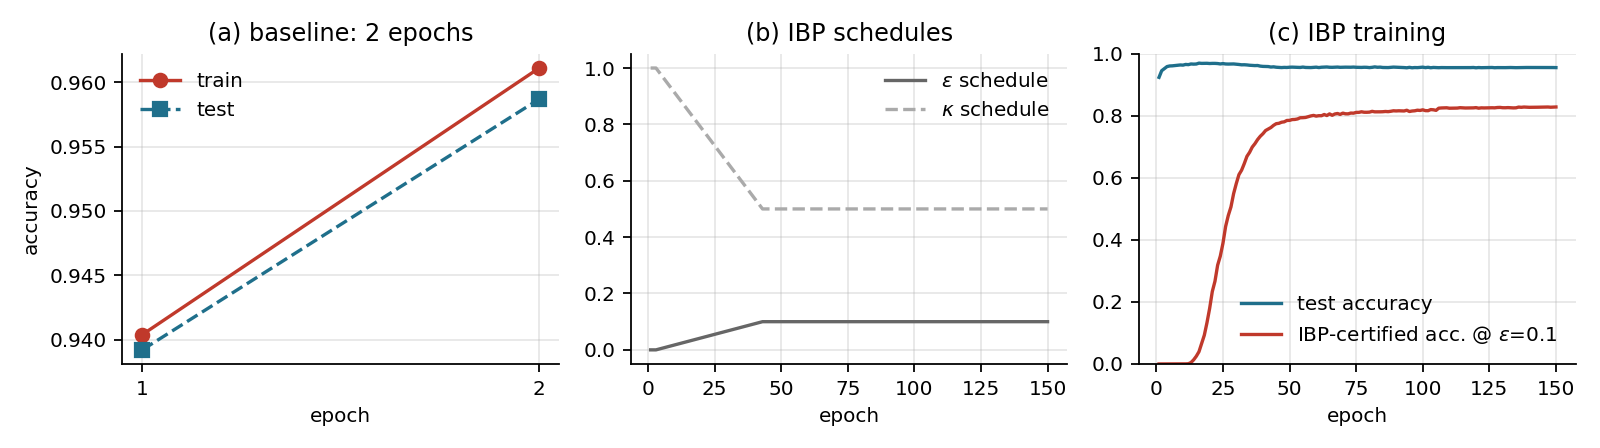
\includegraphics[width=\textwidth]{fig_training.png}
\caption{(a) Baseline training. (b) The $\eps$ and $\kappa$ schedules used for
certified training in Step~4. (c) Standard and IBP-certified test accuracy
during certified training; note that certified accuracy is zero until the
$\eps$-ramp begins and then rises smoothly, while clean accuracy is barely
affected.}
\label{fig:training}
\end{figure}

\section{Step 2 --- Attacking the model with FGSM}

\subsection{Method}
FGSM~\cite{goodfellow2015} takes a single step of size $\eps$ in the direction
that maximises the training loss, using the sign of the input gradient because
that is the steepest-ascent direction under an $\ell_\infty$ constraint:
\begin{equation}
x_{\mathrm{adv}} \;=\; \Pi_{[0,1]}\Bigl(x + \eps\,\mathrm{sign}\bigl(\nabla_x \mathcal{L}(f(x),c)\bigr)\Bigr).
\label{eq:fgsm}
\end{equation}
It is a \emph{linearisation} attack: it assumes the loss is approximately
affine over $\B_\eps(x)$. It is therefore cheap but not optimal, and we also
report PGD~\cite{madry2018} --- iterated FGSM with projection and random
restarts --- as a strictly stronger reference. Any input on which either attack
succeeds is definitively non-robust.

\subsection{Results and the choice of $\eps^\star$}

\begin{table}[H]
\centering\small
\begin{tabular}{lrrrrrrrrr}
\toprule
$\eps$ & $0.01$ & $0.02$ & $0.03$ & $0.05$ & $0.075$ & $\mathbf{0.10}$ & $0.15$ & $0.20$ & $0.30$\\
\midrule
accuracy under FGSM & $92.34$ & $87.01$ & $79.13$ & $54.91$ & $24.69$ & $\mathbf{8.92}$ & $0.84$ & $0.10$ & $0.00$\\
newly fooled (\% of test set) & $3.43$ & $8.76$ & $16.64$ & $40.86$ & $71.08$ & $\mathbf{86.85}$ & $94.93$ & $95.67$ & $95.77$\\
\bottomrule
\end{tabular}
\caption{FGSM against the baseline model (clean accuracy $95.77\%$). ``Newly
fooled'' counts test images that were classified correctly and became incorrect.}
\label{tab:fgsm}
\end{table}

Following the phrasing of the assignment, a representative statement of the
result is: \emph{adding noise of magnitude $\eps=0.05$ causes misclassification
of $40.86\%$ of the test samples that were previously correct; at
$\eps=0.1$ this rises to $86.85\%$.} We adopt
\[
\boxed{\eps^\star = 0.1}
\]
as the operating point for Steps~3--6. Three reasons: (i) it is the canonical
$\ell_\infty$ benchmark for MNIST, so our certified numbers are comparable with
the literature; (ii) it destroys the baseline unambiguously ($95.77\%\to8.92\%$
under FGSM, $\to3.13\%$ under PGD-50), which makes Step~3's proof of weakness
non-controversial; and (iii) it is large enough that certified training is
genuinely challenging rather than trivial.

At $\eps^\star$ the attack fools $\mathbf{8685}$ test images
($90.69\%$ of all correctly classified ones). Their indices, clean images,
adversarial images, true labels and adversarial predictions are stored in
\texttt{results/fooled\_samples.npz} and re-used in Step~5, as required.
Figure~\ref{fig:examples} shows a representative selection: the perturbations
are structured (they trace the stroke boundaries) but semantically meaningless
to a human observer.

\begin{figure}[H]
\centering
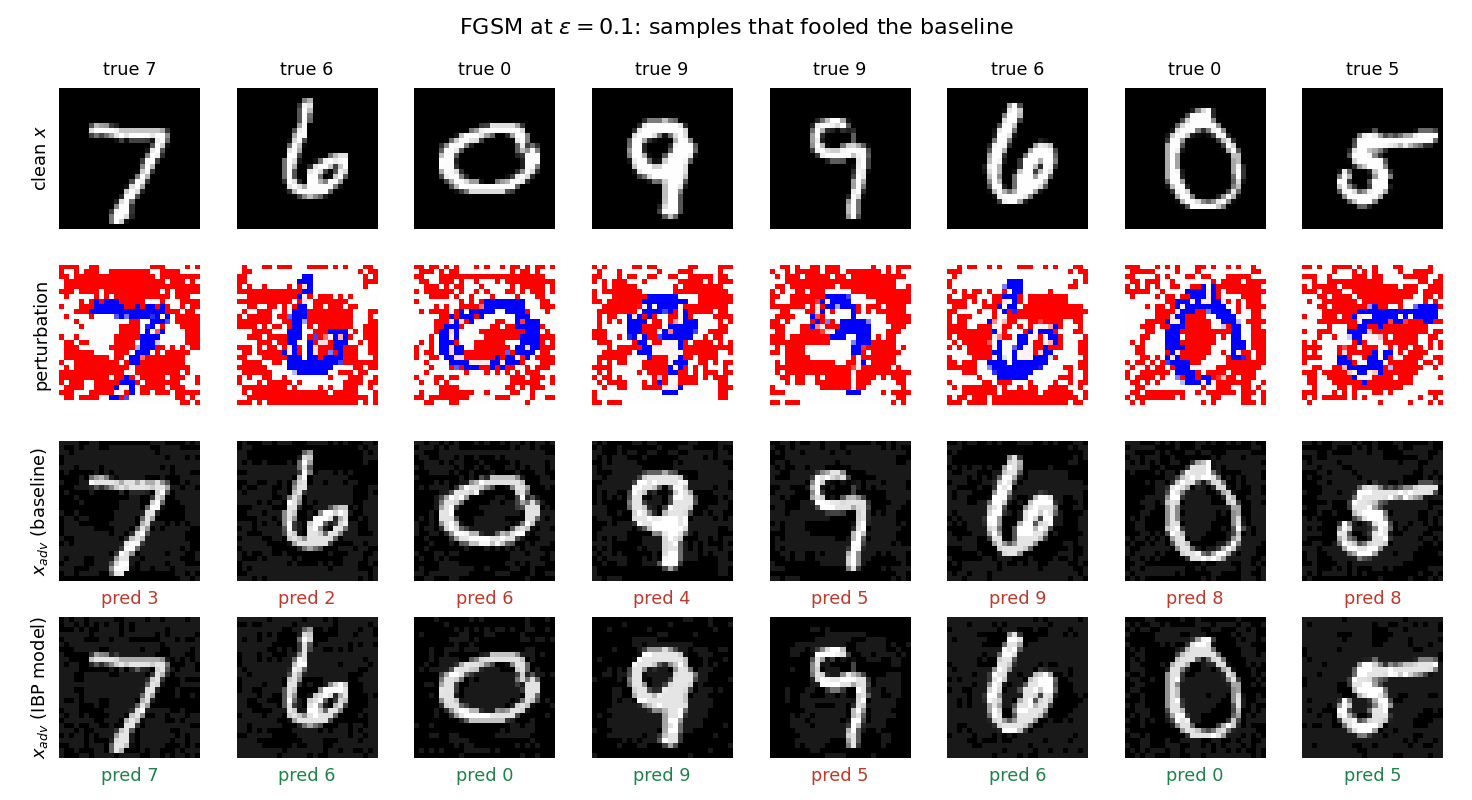
\includegraphics[width=0.92\textwidth]{fig_examples.png}
\caption{Eight of the $8685$ test images that FGSM flips on the baseline model
at $\eps=0.1$. Row 1: clean input. Row 2: the perturbation
$\eps\,\mathrm{sign}(\nabla_x\mathcal{L})$ (red/blue $=\pm\eps$). Row 3: the
adversarial input and the baseline's (wrong) prediction. Row 4: the same attack
re-crafted against the IBP-trained model of Step~4 --- green labels are
recovered predictions (Step~5).}
\label{fig:examples}
\end{figure}

\section{Step 3 --- Proving the weakness formally}

\subsection{The specification}
Property~\eqref{eq:spec} is equivalent to positivity of the worst-case margin
\begin{equation}
m^\star(x,c) \;=\; \min_{j\neq c}\;\min_{x'\in\B_\eps(x)}\;\bigl(z_c(x')-z_j(x')\bigr) \;>\; 0 ,
\label{eq:margin}
\end{equation}
where $z=f(x')$ are the logits. Every verifier below computes a \emph{lower
bound} $\lb{m}\le m^\star$; if $\lb{m}>0$ the input is certified robust. Only
the MILP verifier computes $m^\star$ exactly.

\subsection{Three sound abstract domains}

\paragraph{(a) Interval / IBP (the box domain).}
Bounds are propagated element-wise. For an affine layer $z = a W + b$ we use the
numerically stable midpoint--radius form, which is \emph{exact} for a box input:
\begin{equation}
\mu=\tfrac{\lb{a}+\ub{a}}{2},\quad r=\tfrac{\ub{a}-\lb{a}}{2},\qquad
\lb{z}= \mu W + b - r|W|,\qquad
\ub{z}= \mu W + b + r|W| .
\label{eq:ibp}
\end{equation}
ReLU is monotone, so $[\lb{z},\ub{z}]\mapsto[\mathrm{relu}(\lb{z}),\mathrm{relu}(\ub{z})]$
is exact too. The imprecision comes entirely from \emph{losing the correlations
between neurons}: after the first layer the box treats all $64$ activations as
independent, whereas they are all functions of the same $784$ inputs.

\paragraph{(b) Zonotope / DeepZono~\cite{singh2018}.}
A zonotope $\hat a = a_0 + \sum_i g_i\epsilon_i$, $\epsilon_i\in[-1,1]$, keeps
those correlations: affine layers act exactly on the generators $g_i$. Only ReLU
loses information. For a \emph{crossing} unit ($\lb{z}<0<\ub{z}$) the
area-minimal transformer is
\begin{equation}
\hat y = \lambda \hat z + \mu + \mu\,\epsilon_{\text{new}},\qquad
\lambda=\frac{\ub{z}}{\ub{z}-\lb{z}},\qquad \mu = -\frac{\lambda\lb{z}}{2},
\end{equation}
which introduces one fresh noise symbol per unstable neuron.

\paragraph{(c) DeepPoly / CROWN~\cite{singh2019,zhang2018}.}
Each ReLU is bounded by two affine functions of its own pre-activation,
\begin{equation}
\lambda\, z \;\le\; \mathrm{relu}(z) \;\le\; \frac{\ub{z}}{\ub{z}-\lb{z}}\,(z-\lb{z}),
\qquad \lambda\in[0,1],
\label{eq:relax}
\end{equation}
and the resulting linear expressions are \emph{back-substituted} all the way to
the input layer before being concretised over the input box. Writing the
objective as $A^{(L)}z^{(L)}+d$, the recursion through a ReLU splits on the sign
of each coefficient (positive coefficients use the lower relaxation, negative
ones the upper), and through an affine layer it is exact. We use the
area-minimising heuristic $\lambda=\mathbb{1}[\ub{z}\ge-\lb{z}]$, which is
exactly ERAN's DeepPoly rule and CROWN's adaptive rule; with this choice
\emph{the two tools compute identical bounds on a feed-forward ReLU network},
which is why re-implementing one of them suffices.

\begin{remark}[Intersection with the box]
Because the lower relaxation in~\eqref{eq:relax} can dip below the trivial bound
$\mathrm{relu}(z)\ge0$, neither the zonotope nor DeepPoly \emph{dominates} the box
domain a priori. Both ERAN and \texttt{auto\_LiRPA} therefore keep the tighter of
the two at every layer, and so do we. Without this intersection we measured
DeepPoly bounds that were occasionally \emph{worse} than plain intervals.
\end{remark}

\begin{remark}[DeepZono vs.\ DeepPoly]
Our randomised cross-checks confirm the known theoretical result that the two
domains are \emph{incomparable}: on random networks each is sometimes tighter.
On the real network DeepPoly wins on average (Table~\ref{tab:sweep}).
\end{remark}

\subsection{A complete verifier: mixed-integer programming}
Sound-but-incomplete answers leave ``unknown'' cases, so we additionally encode
the exact problem as a MILP~\cite{tjeng2019}. Each unstable ReLU
$a=\mathrm{relu}(z)$ with $\lb{z}<0<\ub{z}$ becomes, with $\delta\in\{0,1\}$,
\begin{equation}
a\ge 0,\qquad a\ge z,\qquad a\le \ub{z}\,\delta,\qquad a\le z-\lb{z}(1-\delta),
\end{equation}
which is an exact ``big-M'' encoding; stable units are substituted away. The
tighter the pre-activation bounds $\lb{z},\ub{z}$, the tighter the relaxation, so
we feed the DeepPoly bounds into the encoding. Rather than \emph{minimising} the
margin we solve a \emph{feasibility} problem per target class $j$ --- ``does
there exist $x'\in\B_\eps(x)$ with $z_j\ge z_c$?'' --- because the solver may
then stop as soon as infeasibility is proven instead of closing an optimality
gap; on our instances this was roughly an order of magnitude faster, and we
verified that both formulations always agree.

\subsection{Validation of the implementation}
Before trusting any number we checked, on random networks with $8$ inputs and
$4$ classes, that (i)~all three abstract domains give bounds below the exact
MILP optimum, (ii)~the MILP optimum lies below the best margin found by
$150\,000$ random samples per input, and (iii)~the feasibility and optimisation
MILP formulations agree on every instance. All checks passed.

\subsection{Results}

\begin{table}[H]
\centering\small
\begin{tabular}{lrrrrrr}
\toprule
& \multicolumn{6}{c}{certified accuracy (\%) on the first 100 test images}\\
\cmidrule(l){2-7}
$\eps$ & $0.01$ & $0.02$ & $0.03$ & $0.05$ & $0.075$ & $0.10$\\
\midrule
\multicolumn{7}{l}{\emph{baseline model} (clean accuracy on this subset: $99\%$)}\\
\quad PGD-50 (upper bound on robustness) & $98$ & $91$ & $78$ & $40$ & $8$ & $1$\\
\quad Interval / IBP  & $0$  & $0$  & $0$  & $0$ & $0$ & $0$\\
\quad DeepZono        & $95$ & $82$ & $39$ & $5$ & $0$ & $0$\\
\quad DeepPoly / CROWN& $95$ & $83$ & $44$ & $5$ & $0$ & $0$\\
\midrule
\multicolumn{7}{l}{\emph{IBP-trained model} (Step~4; clean accuracy on this subset: $99\%$)}\\
\quad PGD-50 (upper bound on robustness) & $98$ & $98$ & $97$ & $96$ & $93$ & $87$\\
\quad Interval / IBP   & $98$ & $98$ & $97$ & $95$ & $91$ & $82$\\
\quad DeepZono         & $98$ & $98$ & $97$ & $95$ & $91$ & $82$\\
\quad DeepPoly / CROWN & $98$ & $98$ & $97$ & $95$ & $91$ & $82$\\
\bottomrule
\end{tabular}
\caption{Certified accuracy versus perturbation budget. PGD gives an upper bound
on the true robust accuracy; the abstract domains give lower bounds. The true
value lies between them.}
\label{tab:sweep}
\end{table}

At $\eps^\star=0.1$ the verdict on the baseline is unambiguous
(Table~\ref{tab:complete}): \textbf{no test input at all can be certified by any
domain}, $98$ of $100$ are \emph{definitively falsified} by an explicit
counterexample, one is already misclassified without any perturbation, and a
single instance (index~82) remained undecided within the $30$~s MILP budget.
For that instance a very strong targeted PGD attack ($30$ restarts $\times$
$400$ steps $\times$ $9$ target classes) could not push the margin below
$+2.41$, so it is most likely robust; we report it honestly as
\textsc{timeout} rather than claiming a proof. Since a robust point contributes
at most one percentage point, the conclusion --- certified accuracy
$\in[0\%,1\%]$ --- is unaffected.

The $\eps$-sweep is more informative than the single operating point. At
$\eps=0.03$ PGD leaves $78\%$ accuracy while DeepPoly certifies only $44\%$: a
$34$-point \emph{incompleteness gap}. This is the characteristic signature of a
normally trained network --- it is not that the network is non-robust there, it
is that the abstraction is too coarse to prove it. Note also that the interval
domain certifies \emph{nothing at all}, even at $\eps=0.01$: after two affine
layers the accumulated radius $r|W_1||W_2|$ already dwarfs the logit gaps.

\begin{table}[H]
\centering\small
\begin{tabular}{lrr}
\toprule
& baseline & IBP-trained\\
\midrule
clean accuracy (100-image subset) & $99$ & $99$\\
certified robust --- interval / DeepZono / DeepPoly & $0$ / $0$ / $0$ & $82$ / $82$ / $82$\\
\textbf{complete (MILP) robust} & $\mathbf{0}$ & $\mathbf{82}$\\
falsified (explicit counterexample) & $98$ & $17$\\
\quad of which found by PGD / by MILP & $98$ / $0$ & $13$ / $4$\\
misclassified without perturbation & $1$ & $1$\\
undecided (30\,s MILP timeout) & $1$ & $0$\\
\midrule
unstable ReLUs per input (mean, of 96) & $81.7$ & $12.8$\\
\quad layer 1 (of 64) / layer 2 (of 32) & $52.0$ / $29.7$ & $7.4$ / $5.5$\\
median width of the 10 output bounds --- IBP & $124.8$ & $3.76$\\
median width of the 10 output bounds --- DeepPoly & $36.5$ & $3.68$\\
\midrule
runtime, 100 inputs --- interval / DeepZono / DeepPoly & $0.002$ / $0.08$ / $0.48$ s & $0.002$ / $0.08$ / $0.46$ s\\
runtime, MILP phase & $30.5$ s (1 input) & $3.5$ s (4 inputs)\\
\bottomrule
\end{tabular}
\caption{Complete verification results at $\eps^\star=0.1$ (Steps~3 and~6).}
\label{tab:complete}
\end{table}

\section{Step 4 --- Certified training with IBP}
\label{sec:ibp}

\subsection{From bounds to a loss}
Ordinary training minimises $\mathcal{L}(f(x),c)$ at the single point $x$.
Adversarial training replaces $x$ by an attacked $\tilde x$, which improves
empirical robustness but certifies nothing --- it optimises against \emph{one}
point of $\B_\eps(x)$, chosen by a heuristic. IBP training instead pushes the
\emph{whole box} through the network using~\eqref{eq:ibp} and optimises the
worst case over the resulting bounds. This is the crucial conceptual step: the
quantity being minimised is the same quantity a verifier will later try to
certify.

Propagating $\B_\eps(x)$ yields per-logit bounds
$\lb{z}_k\le z_k(x')\le\ub{z}_k$ valid for \emph{all} $x'\in\B_\eps(x)$. Now
consider the specification~\eqref{eq:margin}. For the true class we need the
smallest value it can take, and for every wrong class the largest:
\begin{equation}
\hat z_k \;=\;
\begin{cases}
\lb{z}_c = z_{\min}[c], & k=c \quad\text{(the attacker's best attempt to \emph{lower} the correct score)},\\[2pt]
\ub{z}_k = z_{\max}[k], & k\neq c \quad\text{(the attacker's best attempt to \emph{raise} a wrong score)} .
\end{cases}
\label{eq:zhat}
\end{equation}
This is exactly the construction requested in the assignment. Compactly,
$\hat z = \mu^{(3)} + s\odot r^{(3)}$ with $s_c=-1$ and $s_j=+1$ otherwise,
where $\mu^{(3)},r^{(3)}$ are the midpoint and radius of the logit box.

\begin{proposition}[Soundness]
If $\arg\max_k \hat z_k = c$ then $x$ satisfies~\eqref{eq:spec}.
\end{proposition}
\begin{proof}
For any $x'\in\B_\eps(x)$ and any $j\neq c$ we have
$z_c(x')-z_j(x') \ge \lb{z}_c-\ub{z}_j = \hat z_c-\hat z_j$. If $\hat z_c$ is the
strict maximum of $\hat z$, the right-hand side is positive for every $j$, hence
so is the left-hand side.
\end{proof}

\begin{remark}[Why this is conservative, not exact]
The ten entries of $\hat z$ are attained by ten \emph{different} adversarial
inputs in general; no single $x'$ realises them simultaneously. $\hat z$ is
therefore a pessimistic ``virtual adversary'' that is at least as strong as any
real one. This is precisely what makes the resulting certificate valid --- and
also why certified accuracy is a lower bound on true robust accuracy.
\end{remark}

\subsection{Why cross-entropy on $\hat z$}
Given $\hat z$, the loss is
\begin{equation}
\mathcal{L}_{\mathrm{rob}}(x,c) \;=\; \mathrm{CE}\bigl(\hat z, c\bigr)
\;=\; -\log\frac{e^{\hat z_c}}{\sum_k e^{\hat z_k}}
\;=\; \log\Bigl(1+\textstyle\sum_{j\neq c} e^{-(\hat z_c-\hat z_j)}\Bigr).
\label{eq:robloss}
\end{equation}
Four properties motivate this specific choice over the obvious alternatives
(e.g.\ a hinge $\sum_j\max(0,\gamma-(\hat z_c-\hat z_j))$ or a min-margin loss):

\begin{enumerate}[label=(\roman*)]
\item \textbf{It upper-bounds the verified error.} The rightmost form
in~\eqref{eq:robloss} shows $\mathcal{L}_{\mathrm{rob}}$ is a decreasing,
convex, smooth function of the certified margins
$\hat m_j = \hat z_c-\hat z_j = \lb{z}_c-\ub{z}_j$. Moreover
$\mathcal{L}_{\mathrm{rob}}\ge \log 2\cdot\mathbb{1}[\exists j:\hat m_j\le 0]$,
so minimising it minimises a smooth surrogate of the quantity we actually care
about --- the fraction of inputs a verifier will fail to certify.
\item \textbf{It degenerates gracefully to ordinary training.} At $\eps=0$ the
box collapses, $r^{(3)}=0$, and $\hat z = z$, so~\eqref{eq:robloss} becomes the
standard cross-entropy. This is what allows a single objective and a continuous
$\eps$ ramp (Section~\ref{sec:sched}); a hinge loss would introduce a second,
unrelated hyper-parameter $\gamma$ whose correct scale changes as $\eps$ grows.
\item \textbf{It allocates gradient adaptively across the nine wrong classes.}
$\partial\mathcal{L}_{\mathrm{rob}}/\partial \hat z_j = \mathrm{softmax}(\hat z)_j$,
so the currently most threatening class receives most of the gradient, and
classes that are already far away receive almost none. A sum of hinges treats
all nine equally and wastes capacity; a pure $\min_j$ loss is non-smooth and
gives gradient to only one class per step, which we found trains noticeably
slower.
\item \textbf{It cannot be satisfied trivially.} Because
$\hat z_c-\hat z_j=\lb{z}_c-\ub{z}_j$ depends on the bound \emph{radii}, the only
way to reduce~\eqref{eq:robloss} is to shrink $r^{(3)}$ --- i.e.\ to make the
network genuinely less sensitive over the box --- or to increase the nominal
logit gap. Both are desirable.
\end{enumerate}

\subsection{The mixed objective and the schedules}
\label{sec:sched}
Training on $\mathcal{L}_{\mathrm{rob}}$ alone, at full $\eps$, from a random
initialisation, fails: we measured a median output-bound width of $\sim\!125$ at
initialisation, so $\hat z$ is dominated by the radius term, every class looks
equally bad, and the fastest way to reduce the loss is to drive all weights to
zero --- the network collapses to a constant classifier. Following Gowal
et al.~\cite{gowal2018} we therefore use
\begin{equation}
\mathcal{L} \;=\; \kappa\,\mathrm{CE}\bigl(f(x),c\bigr) \;+\; (1-\kappa)\,\mathrm{CE}\bigl(\hat z(\eps_t),c\bigr),
\end{equation}
with $\eps_t$ ramped linearly $0\to\eps^\star$ and $\kappa$ annealed $1\to0.5$
over the same window (3 warm-up epochs, then a 40-epoch ramp, then 107 epochs at
the final setting; Adam, $\eta=5\times10^{-4}$ decayed $\times0.2$ at $70\%$ and
$90\%$ of training). The $\kappa$ term preserves clean accuracy and keeps the
logits well-scaled; the $\eps$ ramp means the network is never asked to satisfy
a constraint it cannot yet meet. Figure~\ref{fig:training}(b,c) shows the effect:
certified accuracy tracks the ramp smoothly and clean accuracy never drops.

\subsection{Gradients}
Because the objective contains $|W|$ and midpoint/radius terms, its gradient is
not the standard backprop rule. Differentiating $\hat z = \mu W_3+b_3+s\odot(r|W_3|)$
and recursing gives, for each layer $i$,
\begin{equation}
\frac{\partial \mathcal{L}}{\partial W_i} = \mu_{i}^{\!\top} g^{\mu}_i \;+\; \bigl(r_{i}^{\!\top} g^{r}_i\bigr)\odot\mathrm{sign}(W_i),
\qquad
g^{\mu}_{i-1} = g^{\mu}_i W_i^{\!\top},\qquad
g^{r}_{i-1} = g^{r}_i |W_i|^{\!\top},
\end{equation}
with the ReLU step converting $(g^{\mu},g^{r})$ into gradients on $(\lb{z},\ub{z}
)$ via $\partial\mu/\partial\lb{z}=\partial\mu/\partial\ub{z}=\tfrac12$,
$\partial r/\partial\ub{z}=-\partial r/\partial\lb{z}=\tfrac12$ and the masks
$\mathbb{1}[\lb{z}>0],\mathbb{1}[\ub{z}>0]$. The $\mathrm{sign}(W_i)$ term is the
interesting one: it is the gradient of the bound \emph{radius}, and it is what
actively drives the network towards small $|W|$ in the directions that widen the
box. We validated the full derivation against central finite differences: the
maximum relative error over $150$ randomly probed parameters was
$\mathbf{1.9\times10^{-9}}$ (\texttt{python tas\_lib.py}).

\subsection{Results}
After $150$ epochs ($170$~s) the certified model reaches
$\mathbf{95.63\%}$ clean test accuracy --- statistically indistinguishable from
the baseline's $95.77\%$ --- and $\mathbf{82.89\%}$ IBP-certified test accuracy
at $\eps=0.1$ over the full $10\,000$-image test set. The absence of a clean-accuracy
penalty is worth emphasising: at this $\eps$ and this network size, robustness
is obtained essentially for free, which is not generally true at larger $\eps$.

\section{Step 5 --- FGSM against the certified model}

The assignment asks specifically for the previously fooled samples to be
re-tested. Table~\ref{tab:step5} reports both that subset and the full test set.

\begin{table}[H]
\centering\small
\begin{tabular}{lrr}
\toprule
& baseline & IBP-trained\\
\midrule
\multicolumn{3}{l}{\emph{the $8685$ test images that FGSM flipped in Step~2}}\\
\quad clean accuracy                       & $100.00$ & $97.43$\\
\quad accuracy under FGSM re-crafted at $\eps=0.1$ & $0.00$ & $\mathbf{90.13}$\\
\quad accuracy on the \emph{transferred} baseline adversarial images & --- & $93.10$\\
\quad accuracy under PGD-100                & --- & $88.15$\\
\midrule
\multicolumn{3}{l}{\emph{full test set at $\eps=0.1$}}\\
\quad clean                                 & $95.77$ & $95.63$\\
\quad FGSM                                  & $8.92$  & $\mathbf{88.02}$\\
\quad PGD-50                                & $3.13$  & $86.28$\\
\bottomrule
\end{tabular}
\caption{Step~5. Of the $8685$ inputs that defeated the baseline, the certified
model recovers $\mathbf{7828}$ ($90.13\%$) even when the attack is regenerated
against it; only $857$ remain adversarial.}
\label{tab:step5}
\end{table}

Two observations. First, the attack must be \emph{re-crafted}: the old
adversarial images transfer only partially ($93.10\%$ accuracy), so evaluating a
defence on stale adversarial examples would overstate it --- a classic pitfall.
Second, the gap between FGSM ($88.02\%$) and PGD ($86.28\%$) on the certified
model is only $1.7$ points, versus $5.8$ points on the baseline: gradient masking
is not occurring, and FGSM is a reasonable proxy here. Figure~\ref{fig:fgsm}
shows the full curves; the certified model degrades gracefully and only collapses
well beyond the $\eps$ it was trained for.

\begin{figure}[H]
\centering
\begin{subfigure}{0.42\textwidth}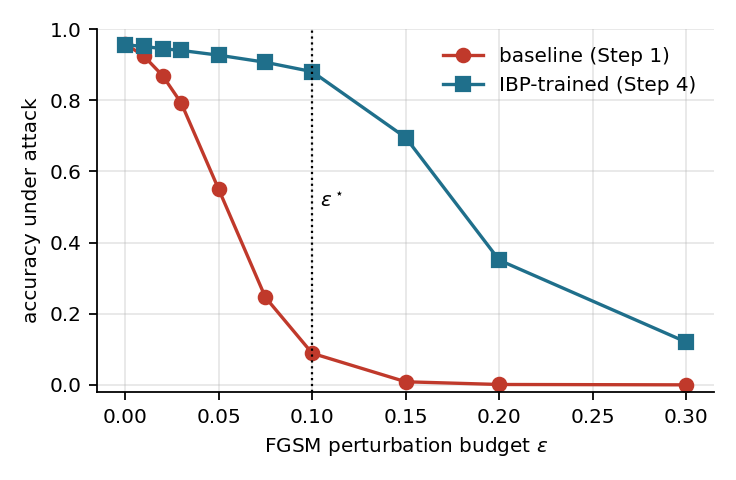
\includegraphics[width=\textwidth]{fig_fgsm_sweep.png}\end{subfigure}
\hfill
\begin{subfigure}{0.56\textwidth}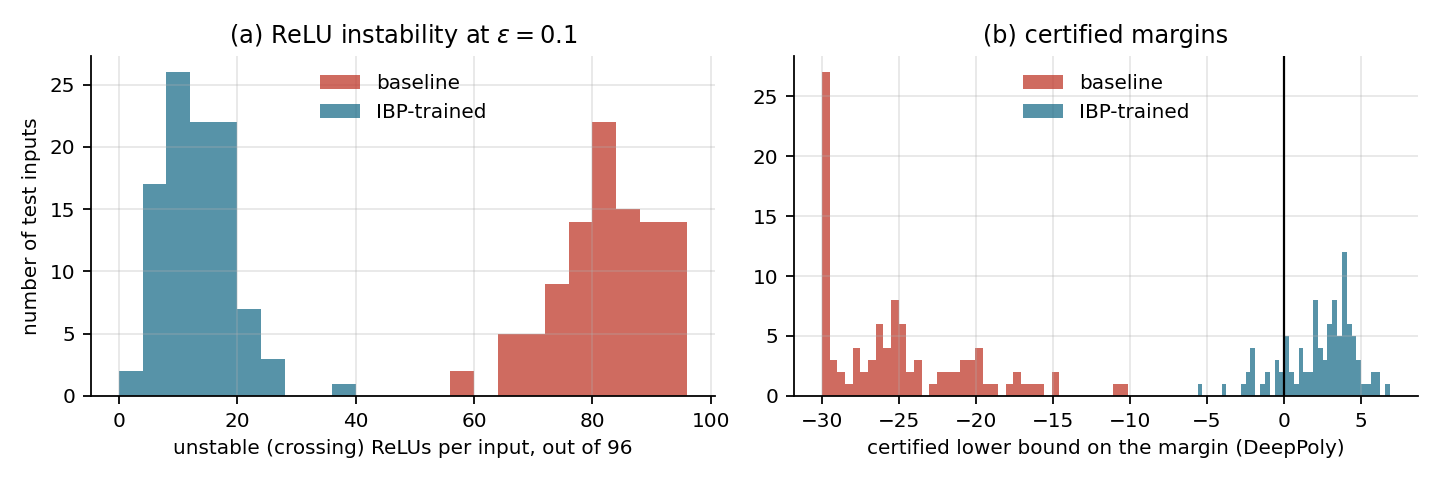
\includegraphics[width=\textwidth]{fig_unstable_margins.png}\end{subfigure}
\caption{Left: accuracy under FGSM versus $\eps$ for both models. Right:
(a)~distribution of unstable ReLUs per input and (b)~certified DeepPoly margins,
at $\eps=0.1$. Certified training moves the margin distribution almost entirely
to the right of zero and roughly halves the input's exposure to ReLU branching.}
\label{fig:fgsm}
\end{figure}

\section{Step 6 --- Verifying the certified model, and why the result changes}

Re-running the entire Step~3 pipeline on the new model gives the right-hand
column of Table~\ref{tab:complete} and Figure~\ref{fig:cert}. Four differences
stand out, and they have a common cause.

\paragraph{1. Certification succeeds, and it is now \emph{exact}.}
$82$ of $100$ inputs are certified, $17$ are falsified by explicit
counterexamples, $1$ is misclassified: the $100$ instances are fully partitioned
with \emph{no} timeouts. Because the MILP verifier is complete, the true robust
accuracy of this model on this subset is exactly $82\%$ --- and DeepPoly reports
exactly $82\%$ as well. \textbf{The incompleteness gap has vanished entirely}
(it was $34$ points on the baseline at $\eps=0.03$). The remaining $5$-point
distance to PGD's $87\%$ is not verifier looseness; it is the difference between
``PGD failed to find an attack'' and ``an attack exists'', and the MILP settles
it in favour of the latter for four inputs that PGD had missed. This is a good
illustration of why an attack is not a substitute for a proof.

\paragraph{2. All three abstract domains agree.}
Interval, DeepZono and DeepPoly certify the identical set of $82$ inputs. On the
baseline they differed enormously ($0\%$ vs.\ $95\%$ at $\eps=0.01$). The reason
is direct: IBP training minimises the \emph{box} bound, so the trained network is
one on which the box abstraction happens to be tight, and the more expensive
domains have nothing left to recover. Quantitatively, the median output-bound
width is $3.76$ for IBP and $3.68$ for DeepPoly --- a $2\%$ improvement, against
a $3.4\times$ improvement ($124.8\to36.5$) on the baseline. In practice this
means the cheapest verifier ($0.002$~s for 100 inputs) is now as good as the
$240\times$ more expensive one.

\paragraph{3. ReLU instability collapses.}
The mean number of unstable ReLUs per input drops from $81.7$ to $12.8$ out of
$96$ ($52.0\to7.4$ in layer 1, $29.7\to5.5$ in layer 2). This is the mechanism
behind both previous points. Every crossing ReLU is a place where the relaxation
must lose information and where the MILP must branch; the exact problem has
$2^{\#\text{unstable}}$ activation patterns, so $2^{81.7}$ becomes $2^{12.8}$.
Correspondingly, the MILP phase took $30.5$~s and still timed out on the
baseline, but resolved four inputs in $3.5$~s on the certified model.

\paragraph{4. Certified training is a regulariser towards \emph{verifiability}.}
Combining the above: IBP training does not only move the decision boundary away
from the data, it reshapes the network so that a cheap over-approximation of it
is accurate. The $\mathrm{sign}(W)$ gradient term of Section~\ref{sec:ibp} makes
this explicit --- it penalises exactly those weights that widen the interval,
pushing pre-activations away from zero and stabilising ReLUs. The price is a
loss of expressive capacity, which at $\eps=0.1$ on MNIST is small enough to be
invisible ($95.77\%\to95.63\%$) but becomes severe at larger $\eps$ or on harder
datasets --- the well-documented accuracy/robustness/verifiability trilemma.

\begin{figure}[H]
\centering
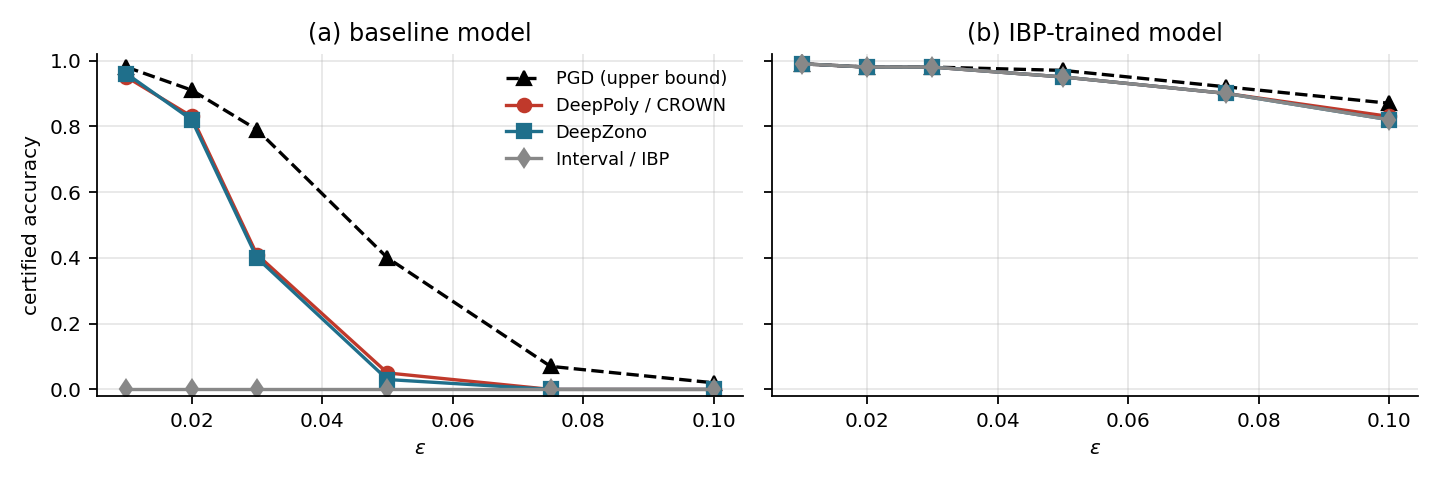
\includegraphics[width=0.86\textwidth]{fig_certified_sweep.png}
\caption{Certified accuracy versus $\eps$. The shaded distance between the
dashed PGD curve and the solid certified curves is the region of uncertainty: on
the baseline (a) it is dominated by verifier incompleteness, on the certified
model (b) it is only $5$ points wide and, at $\eps=0.1$, entirely attributable
to genuinely non-robust inputs rather than to the abstraction.}
\label{fig:cert}
\end{figure}

\begin{figure}[H]
\centering
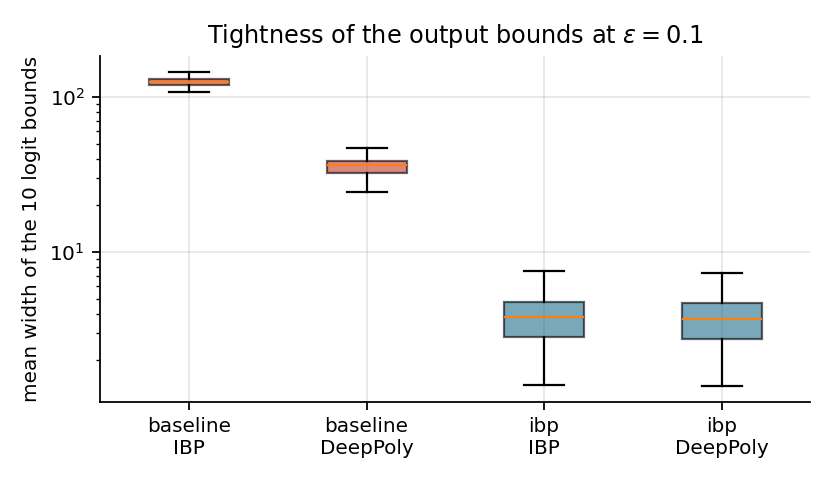
\includegraphics[width=0.5\textwidth]{fig_bound_width.png}
\caption{Width of the propagated logit bounds at $\eps=0.1$ (log scale). On the
baseline, back-substitution (DeepPoly) buys a $3.4\times$ tightening over plain
intervals; after certified training the two are within $2\%$ of each other.}
\label{fig:width}
\end{figure}

\section{Discussion, limitations and conclusions}

\paragraph{What was shown.} A two-epoch MLP with $95.77\%$ test accuracy is not
merely attackable --- it is \emph{provably} non-robust: at $\eps=0.1$ a complete
verifier finds an explicit counterexample for $98$ of $100$ test inputs, and no
abstract domain can certify a single one. Replacing the point-wise loss with the
worst-case-logit IBP loss of~\eqref{eq:zhat}--\eqref{eq:robloss} raises
FGSM accuracy from $8.92\%$ to $88.02\%$ and yields a machine-checked guarantee
for $82\%$ of inputs, at a clean-accuracy cost of $0.14$ points.

\paragraph{Limitations.} (i) Verification statistics are computed on the first
$100$ test images, the convention used by ERAN and CROWN, so they carry a
sampling error of roughly $\pm4$ points; the IBP-certified accuracy over the
full $10\,000$ images ($82.89\%$) agrees closely with the $82\%$ measured on the
subset. (ii) One baseline instance is unresolved (30\,s MILP budget); a longer
budget or LP-based bound tightening would close it. (iii) The guarantee is
\emph{local} --- it says nothing about inputs outside the tested boxes --- and it
concerns $\ell_\infty$ perturbations only, not rotations, occlusions or
distribution shift. (iv) We train at exactly the evaluation $\eps$; training at
$1.1\eps$ is known to buy a further point or two of certified accuracy.
(v)~The ERAN and \texttt{auto\_LiRPA} runs are provided as reproducible scripts
and validated exports rather than executed here, for the environment reasons
given in Section~\ref{sec:env}; our re-implementations were instead validated
against an exact oracle, which is a stronger check than agreement with another
incomplete tool.

\paragraph{Takeaway.} The three families of techniques are complementary and
should be reported together. An attack gives an upper bound on robustness, an
abstract domain gives a lower bound, and only a complete method closes the
interval. Certified training is what makes the lower bound worth computing: it
converts a network on which the cheap analysis is useless into one on which the
cheap analysis is exact.

\section{Reproducibility}

\begin{table}[H]
\centering\footnotesize
\begin{tabular}{@{}p{5.2cm}p{10.3cm}@{}}
\toprule
\texttt{code/tas\_lib.py} & data, network, backprop, Adam, FGSM/PGD, IBP forward + gradients\\
\texttt{code/verifiers.py} & interval, DeepZono, DeepPoly/CROWN, MILP verifiers\\
\texttt{code/verification\_driver.py} & the combined pipeline used by Steps 3 and 6\\
\texttt{code/step1..step6\_*.py} & the six steps of the assignment, in order\\
\texttt{code/run\_all.py} & runs everything end-to-end\\
\texttt{code/export\_models.py} & ONNX export (+ runtime check) and tool scripts\\
\texttt{code/to\_pytorch.py} & converts the NumPy weights to a PyTorch \texttt{.pth}\\
\texttt{code/run\_autolirpa.py}, \texttt{run\_eran.sh} & drivers for the two official tools\\
\texttt{models/mlp\_baseline.\{npz,onnx\}} & the Step-1 model\\
\texttt{models/mlp\_ibp.\{npz,onnx\}} & the Step-4 model\\
\texttt{results/fooled\_samples.npz} & the $8685$ Step-2 adversarial samples\\
\texttt{results/step*.json}, \texttt{results/figures/} & all numbers and figures in this report\\
\bottomrule
\end{tabular}
\caption{Contents of the submission.}
\end{table}

\noindent\sloppy
\texttt{pip install numpy scipy matplotlib onnx onnxruntime} then
\texttt{cd code \&\& python run\_all.py} reproduces every number above
(about 7 minutes on one CPU core; no GPU and no deep-learning framework
required). Running the official tools additionally requires
\texttt{pip install torch auto\_LiRPA} (for \texttt{run\_autolirpa.py}) or the
\texttt{ethsri/eran:cpu} Docker image (for \texttt{run\_eran.sh}).

\begin{thebibliography}{9}\small
\bibitem{goodfellow2015} I.~Goodfellow, J.~Shlens, C.~Szegedy.
\emph{Explaining and Harnessing Adversarial Examples.} ICLR 2015.
\bibitem{madry2018} A.~Madry, A.~Makelov, L.~Schmidt, D.~Tsipras, A.~Vladu.
\emph{Towards Deep Learning Models Resistant to Adversarial Attacks.} ICLR 2018.
\bibitem{singh2018} G.~Singh, T.~Gehr, M.~Mirman, M.~P\"uschel, M.~Vechev.
\emph{Fast and Effective Robustness Certification.} NeurIPS 2018. (DeepZ / ERAN \texttt{deepzono})
\bibitem{singh2019} G.~Singh, T.~Gehr, M.~P\"uschel, M.~Vechev.
\emph{An Abstract Domain for Certifying Neural Networks.} POPL 2019. (DeepPoly / ERAN \texttt{deeppoly})
\bibitem{zhang2018} H.~Zhang, T.-W.~Weng, P.-Y.~Chen, C.-J.~Hsieh, L.~Daniel.
\emph{Efficient Neural Network Robustness Certification with General Activation Functions.} NeurIPS 2018. (CROWN)
\bibitem{xu2020} K.~Xu et al.
\emph{Automatic Perturbation Analysis for Scalable Certified Robustness and Beyond.} NeurIPS 2020. (\texttt{auto\_LiRPA})
\bibitem{tjeng2019} V.~Tjeng, K.~Xiao, R.~Tedrake.
\emph{Evaluating Robustness of Neural Networks with Mixed Integer Programming.} ICLR 2019.
\bibitem{gowal2018} S.~Gowal et al.
\emph{On the Effectiveness of Interval Bound Propagation for Training Verifiably Robust Models.} arXiv:1810.12715, 2018.
\bibitem{zhang2020} H.~Zhang et al.
\emph{Towards Stable and Efficient Training of Verifiably Robust Neural Networks.} ICLR 2020. (CROWN-IBP)
\end{thebibliography}

\end{document}
